\chapter*{General Introduction}
\addcontentsline{toc}{chapter}{General Introduction}

\section*{Context and Problem Statement}

Agriculture is one of the foundations of food security, economic development, and social stability. However, it is also one of the sectors most exposed to climate variability, water scarcity, soil degradation, and increasing production pressure. In many regions, irrigation remains a central factor determining crop quality and yield. When irrigation is applied too late, plants may suffer water stress and productivity may decrease. When irrigation is applied too early or in excessive quantities, water is wasted, soil nutrients may leach, and the cost of operation increases. The challenge is therefore not simply to irrigate, but to irrigate at the right time, with the right quantity, and according to the actual state of the soil, crop, and environment.

Traditional irrigation practices are often based on fixed schedules, manual field observation, or the farmer's experience. These practices remain valuable because farmers possess contextual knowledge of their crops and land. Nevertheless, they can become insufficient when environmental conditions change quickly or when water availability becomes uncertain. Precision agriculture responds to this issue by relying on sensors, communication systems, data processing, and intelligent decision support. Smart irrigation is one of the most important applications of precision agriculture because it directly addresses water-use efficiency and sustainability.

Digital Twin technology offers a more integrated approach. A Digital Twin is not only a dashboard or a static simulation. It is a virtual representation of a physical system, continuously updated using real data, able to simulate future behavior, support decision-making, and potentially influence the physical system through feedback or actuation. In agriculture, Digital Twins can represent farms, plots, irrigation zones, greenhouses, plants, soil profiles, livestock, or agricultural machinery. Their value lies in connecting physical measurements, computational models, prediction algorithms, and operational decisions within a coherent cyber-physical loop.

This Master Diploma report focuses on the scientific part of Agrio. Its purpose is to study the foundations of precision agriculture and smart irrigation, define the concepts and maturity levels of Digital Twins, review the state of the art of agricultural Digital Twins and intelligent irrigation, and synthesize the main gaps that justify the proposed Agrio direction.

\section*{Objectives}

The central research question of this Master report is: how can the literature on Digital Twins, IoT-based smart irrigation, and machine learning irrigation systems be analyzed in order to position Agrio scientifically? This question is divided into secondary questions: what are the main concepts and maturity levels of Digital Twins in agriculture? Which technologies are commonly used in IoT-based smart irrigation systems? How can machine learning support irrigation decision-making? What are the strengths and limitations of current research? Where does the proposed Agrio prototype stand compared with existing works?

The objectives of the Master Diploma report are: to study Digital Twins and smart irrigation systems in the agricultural domain; to present the fundamental concepts of precision agriculture, IoT, artificial intelligence, and simulation; to review existing research on agricultural Digital Twins and irrigation systems; to compare related works according to clear scientific criteria; and to identify the novelty, limitations, and positioning of Agrio.

\section*{Thesis Outline}

The report is organized according to the Master Diploma structure. The front matter contains the acknowledgements, abstracts, and lists. The introduction presents the context, problem statement, objectives, and outline. The background part introduces precision agriculture, smart irrigation, Digital Twins, IoT, and artificial intelligence. The state-of-the-art part reviews Digital Twins in agriculture and irrigation. The synthesis part compares existing works and positions Agrio scientifically. The report ends with a general conclusion.

\begin{figure}[H]
    \centering
    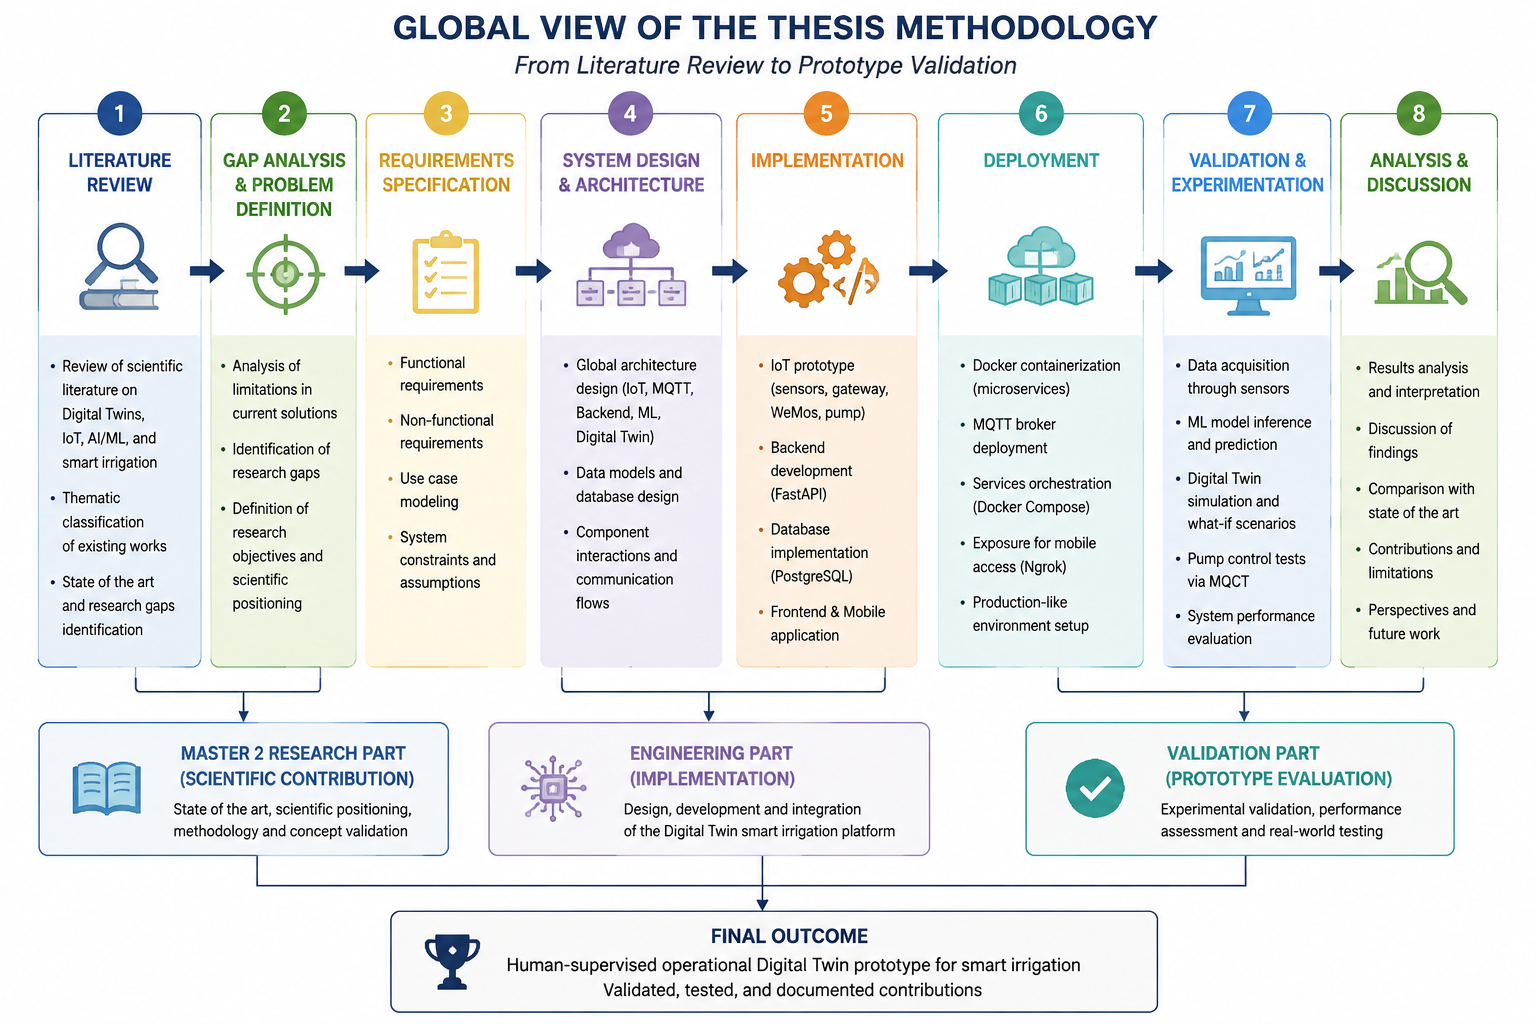
\includegraphics[width=0.9\textwidth]{figures/cover/Figure 0.1 — Global view of the thesis methodology from literature review to prototype validation.png}
    \caption{Global view of the thesis methodology from literature review to prototype validation. Source: Authors.}
    \label{fig:0-1-global-view-of-the-thesis-methodology-from-literature-review-to-pr}
\end{figure}

\begin{footnotesize}
\setlength{\tabcolsep}{2pt}
\begin{longtable}{@{}>{\raggedright\arraybackslash}p{0.28\textwidth}>{\raggedright\arraybackslash}p{0.28\textwidth}>{\raggedright\arraybackslash}p{0.28\textwidth}@{}}
\caption{Summary of Master Diploma objectives and contributions}\\
\toprule
Dimension & Objective & Contribution \\
\midrule
\endfirsthead
\toprule
Dimension & Objective & Contribution \\
\midrule
\endhead
Scientific background & Study Digital Twins, smart irrigation, IoT, and ML concepts & Structured theoretical foundation \\
State of the art & Analyze recent research on agricultural Digital Twins and smart irrigation & Literature review and research gap identification \\
Synthesis & Compare existing systems according to Digital Twin maturity and irrigation functionality & Scientific positioning of Agrio \\
\bottomrule
\end{longtable}
\end{footnotesize}
